\subsection{Speech Recognition with Weighted Finite-State Transducers \cite{Mohri2000}}

This paper describes a general representation and algorithmic framework for speech recognition based on \emph{weighted finite-state transducers (WFST)}. These transducers provide a common and natural representation for major components of speech recognition systems, including \emph{hidden Markov models (HMMs)}, context-dependency models, pronunciation dictionaries, etc. The paper shows the application of the proposed method to large-vocabulary recognition task.

A \emph{finite-state transducer} is a finite automaton whose state transitions are labeled with both input and output symbols. Therefore, a path through the transducer encodes a mapping from an input symbol sequence, or string, to an output string. A weighted transducer puts weights on transitions in addition. In this paper, weights encode the probabilities that accumulates along the path.

\begin{figure}[h]
  \centering
  % Requires \usepackage{graphicx}
  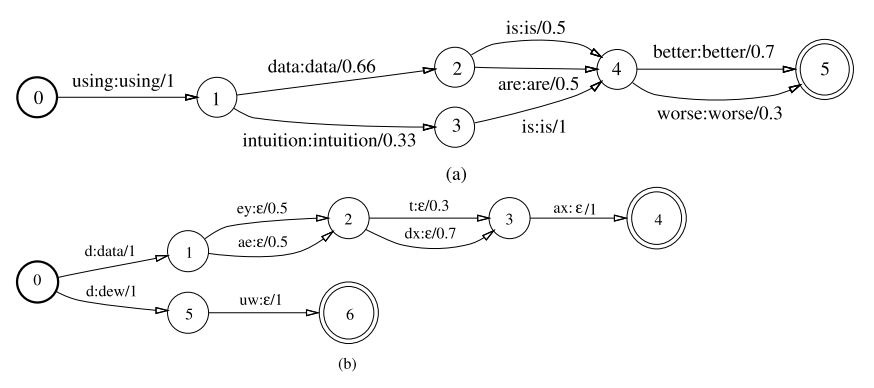
\includegraphics[width=\linewidth]{11_21_WFST.png}\\
  \caption{Examples of weighted finite-state transducer}\label{fig:WFST}
\end{figure}

Figure \ref{fig:WFST} presents a toy language model and a toy pronunciation lexicon as WFSTs. In Figure \ref{fig:WFST}(b), the WFTS maps from phone strings to words in the lexicon, in this example `data' and `dew', with probabilities representing the likelihoods of alternative pronunciations. Similarly, HMM structures can be combined into a single transducer that preserves phone model identity.

The proposed method relies on a common set of weighted transducer operations to combine, optimize, search and prune them. The basic operations \emph{union}, \emph{concatenation}, and \emph{Kleene closure} operations combine transducers in parallel, in series, and with arbitrary repetition, respectively. There are three other key operations that are used in the speech applications:

1) \emph{Composition}: Composition is the transducer operation for combining different levels of representation. For example, a pronunciation lexicon can be composed with a word-level grammar to produce a phone-to-word transducer. In particular, the composition $T = T_1 \circ T_2$ has exactly one path mapping string $u$ to string $w$ for each pair of paths, the first in $T_1$ mapping $u$ to $v$ and the second in $T_2$ mapping $v$ to $w$.

2) \emph{Determinization}: In a deterministic transducer, each state has at most one transition with any given input label and there are no input $\epsilon$-labels. The key advantage of a deterministic transducer is its irredundancy: it contains at most one path matching any given input string, thereby reducing the time and space needed to process the string. The determinization algorithm transforms a non-deterministic WFST into an equivalent deterministic WFST.

3) \emph{Minimization}: Given a deterministic WFST, its size can be reduced by minimization, which can save both space and time. Let the given WFST be denoted as $A$. The minimization algorithm results in a WFST $B$ that is equivalent to $A$, and has the least number of states and the least number of transitions among all deterministic WFSTs equivalent to $A$.

Next we will see how to construct a single recognition transducer that maps from context-dependent phones to a string of words.

Consider the pronunciation lexicon $L$ in Figure \ref{fig:WFST}(b), and the grammar $G$ of Figure \ref{fig:WFST}(a). $L \circ G$ gives a transducer that maps from phones to word strings restricted to the grammar $G$. If we let $C$ represent a transducer from context-dependent phones to context-independent phones, then $C \circ (L \circ G)$ gives a transducer that maps from context-dependent phones (such as triphones) o word strings restricted to the grammar $G$. Finally, the transducer is optimized with determinization and minimization: $N = min(det(C \circ (L \circ G)))$.

In the following sections, the paper introduces the operation algorithms in further details, and reports the experimental results in the large-vocabulary speech recognition task. It is shown that the proposed method can greatly improve the efficiency and save space. 